\begin{figure}
    \centering
    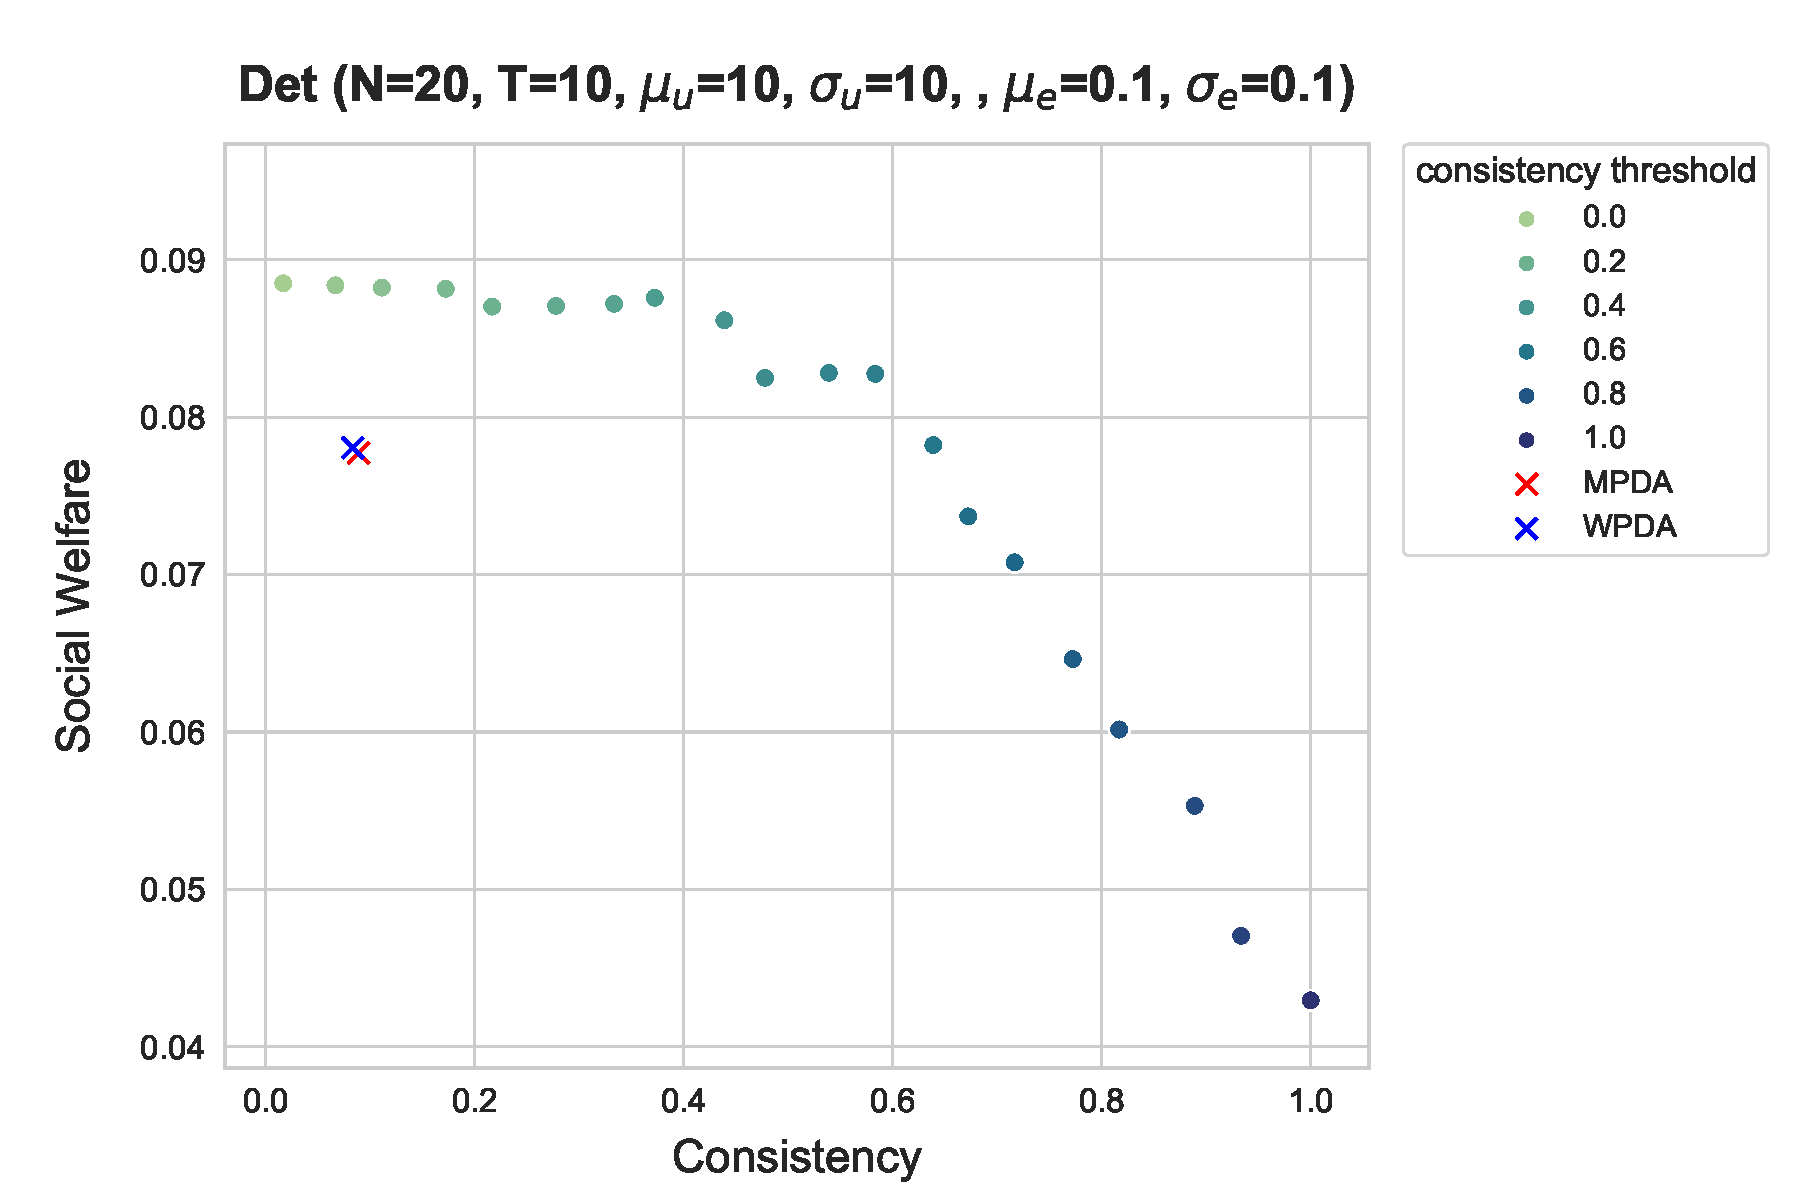
\includegraphics[width=0.32\linewidth]{figures/algs/Det_20_10_10_10.pdf}
    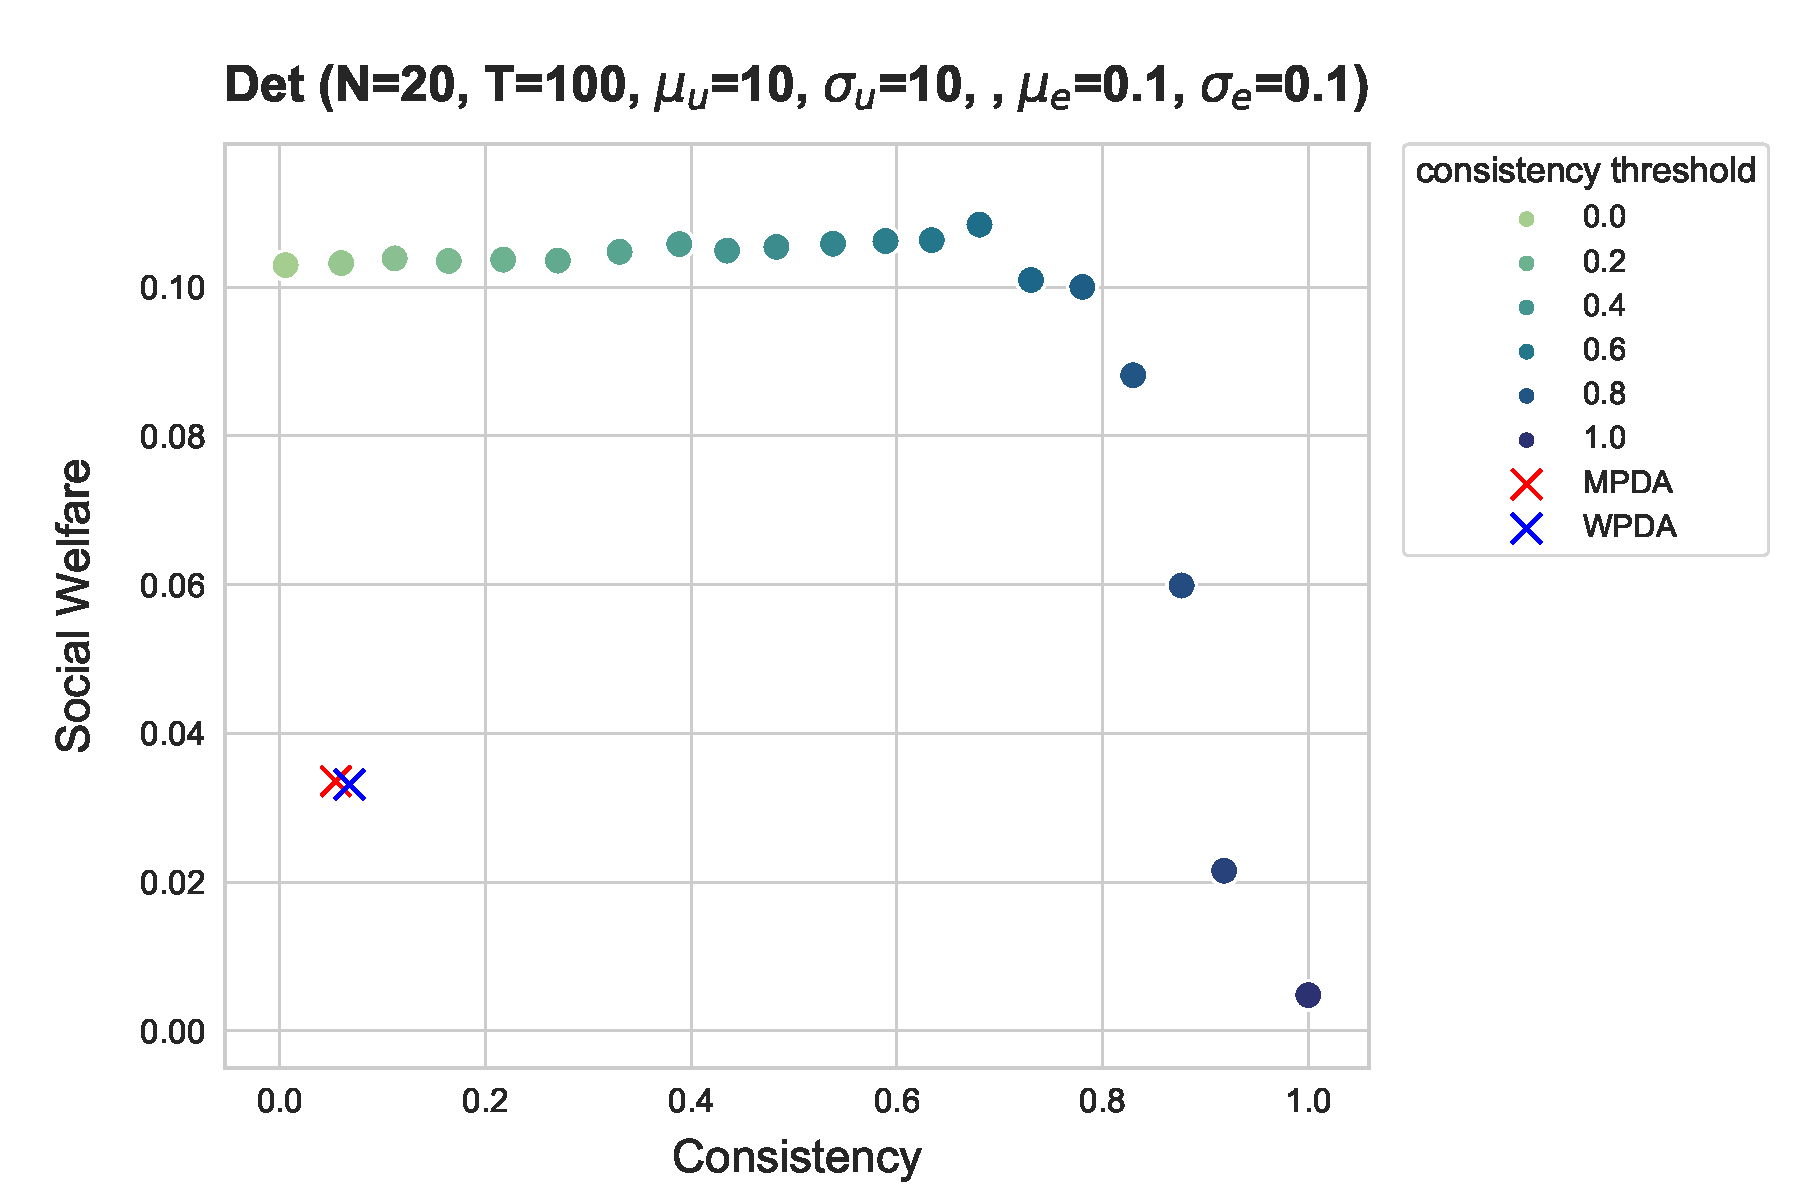
\includegraphics[width=0.32\linewidth]{figures/algs/Det_20_100_10_10.pdf}
    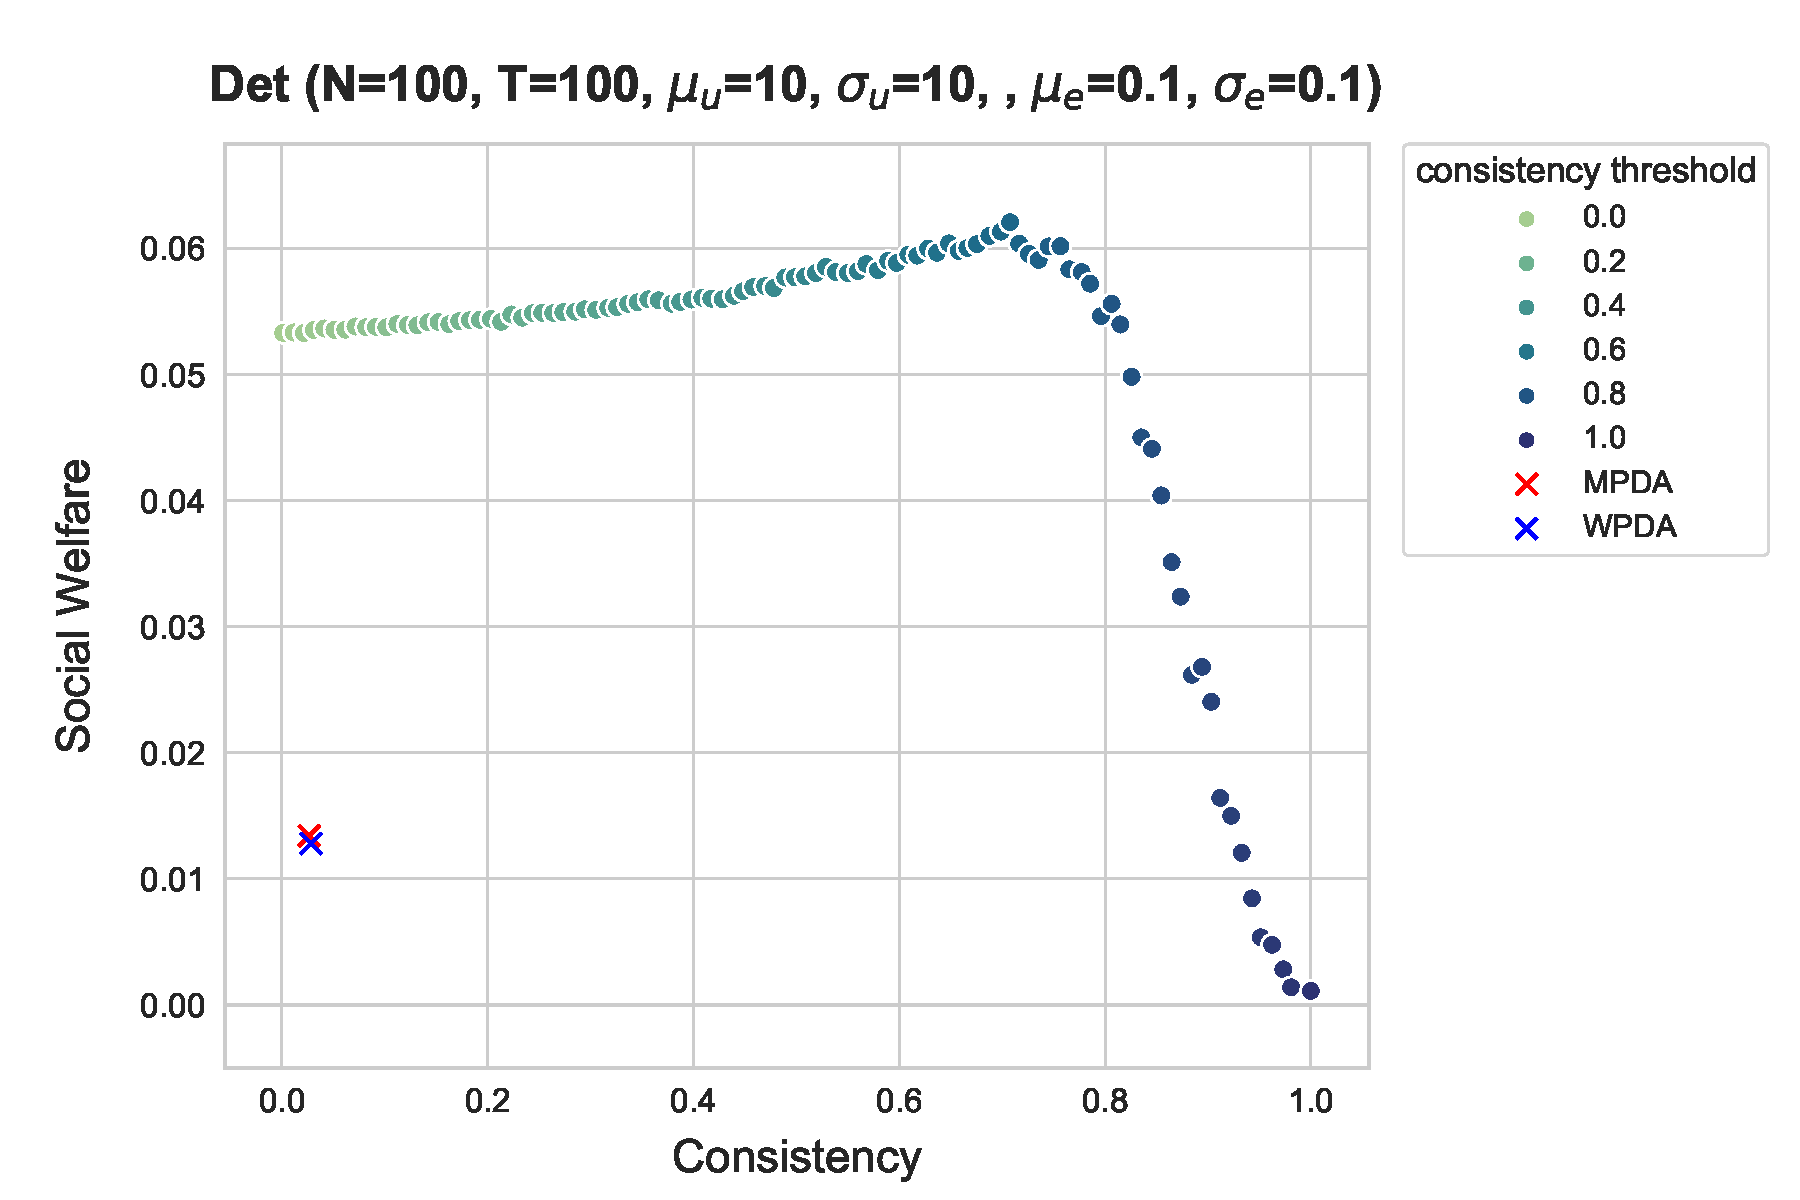
\includegraphics[width=0.32\linewidth]{figures/algs/Det_100_100_10_10.pdf}
    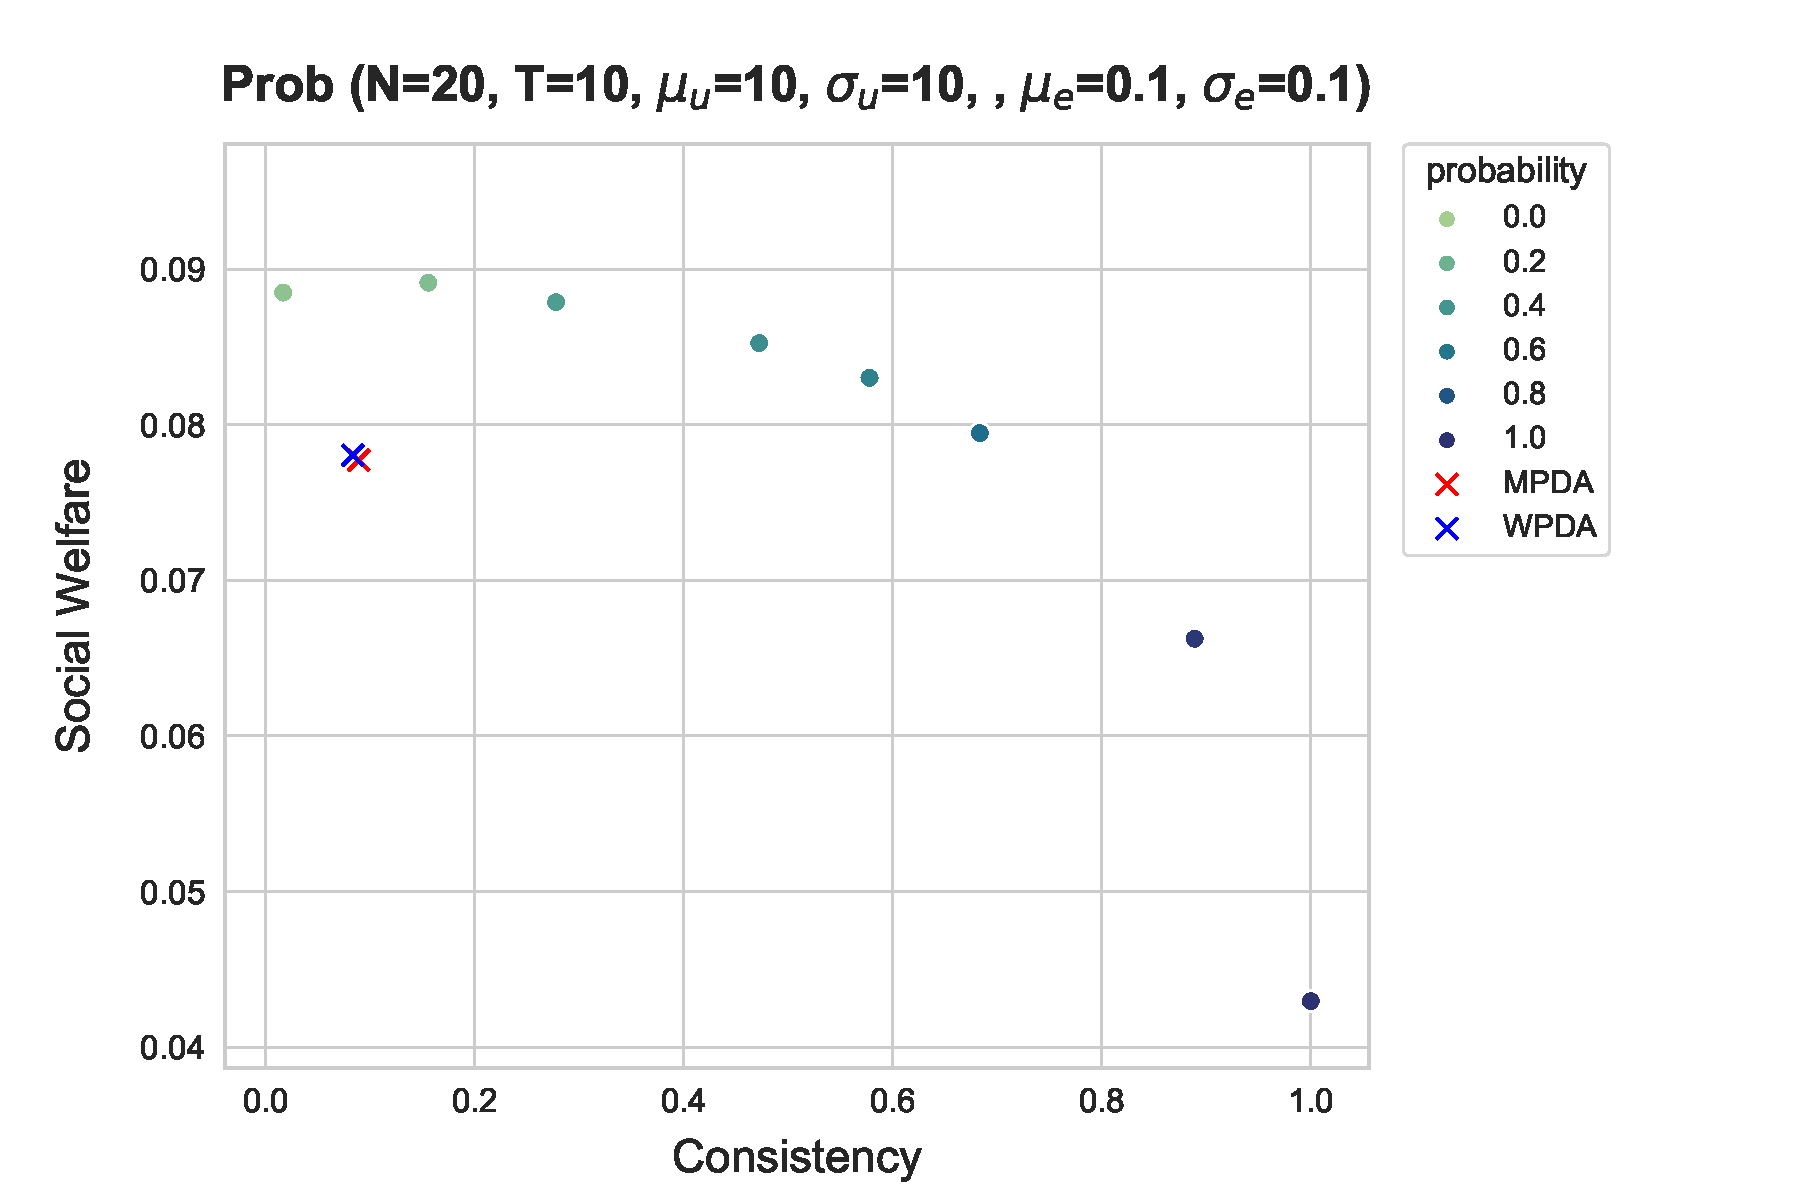
\includegraphics[width=0.32\linewidth]{figures/algs/Prob_20_10_10_10.pdf}
    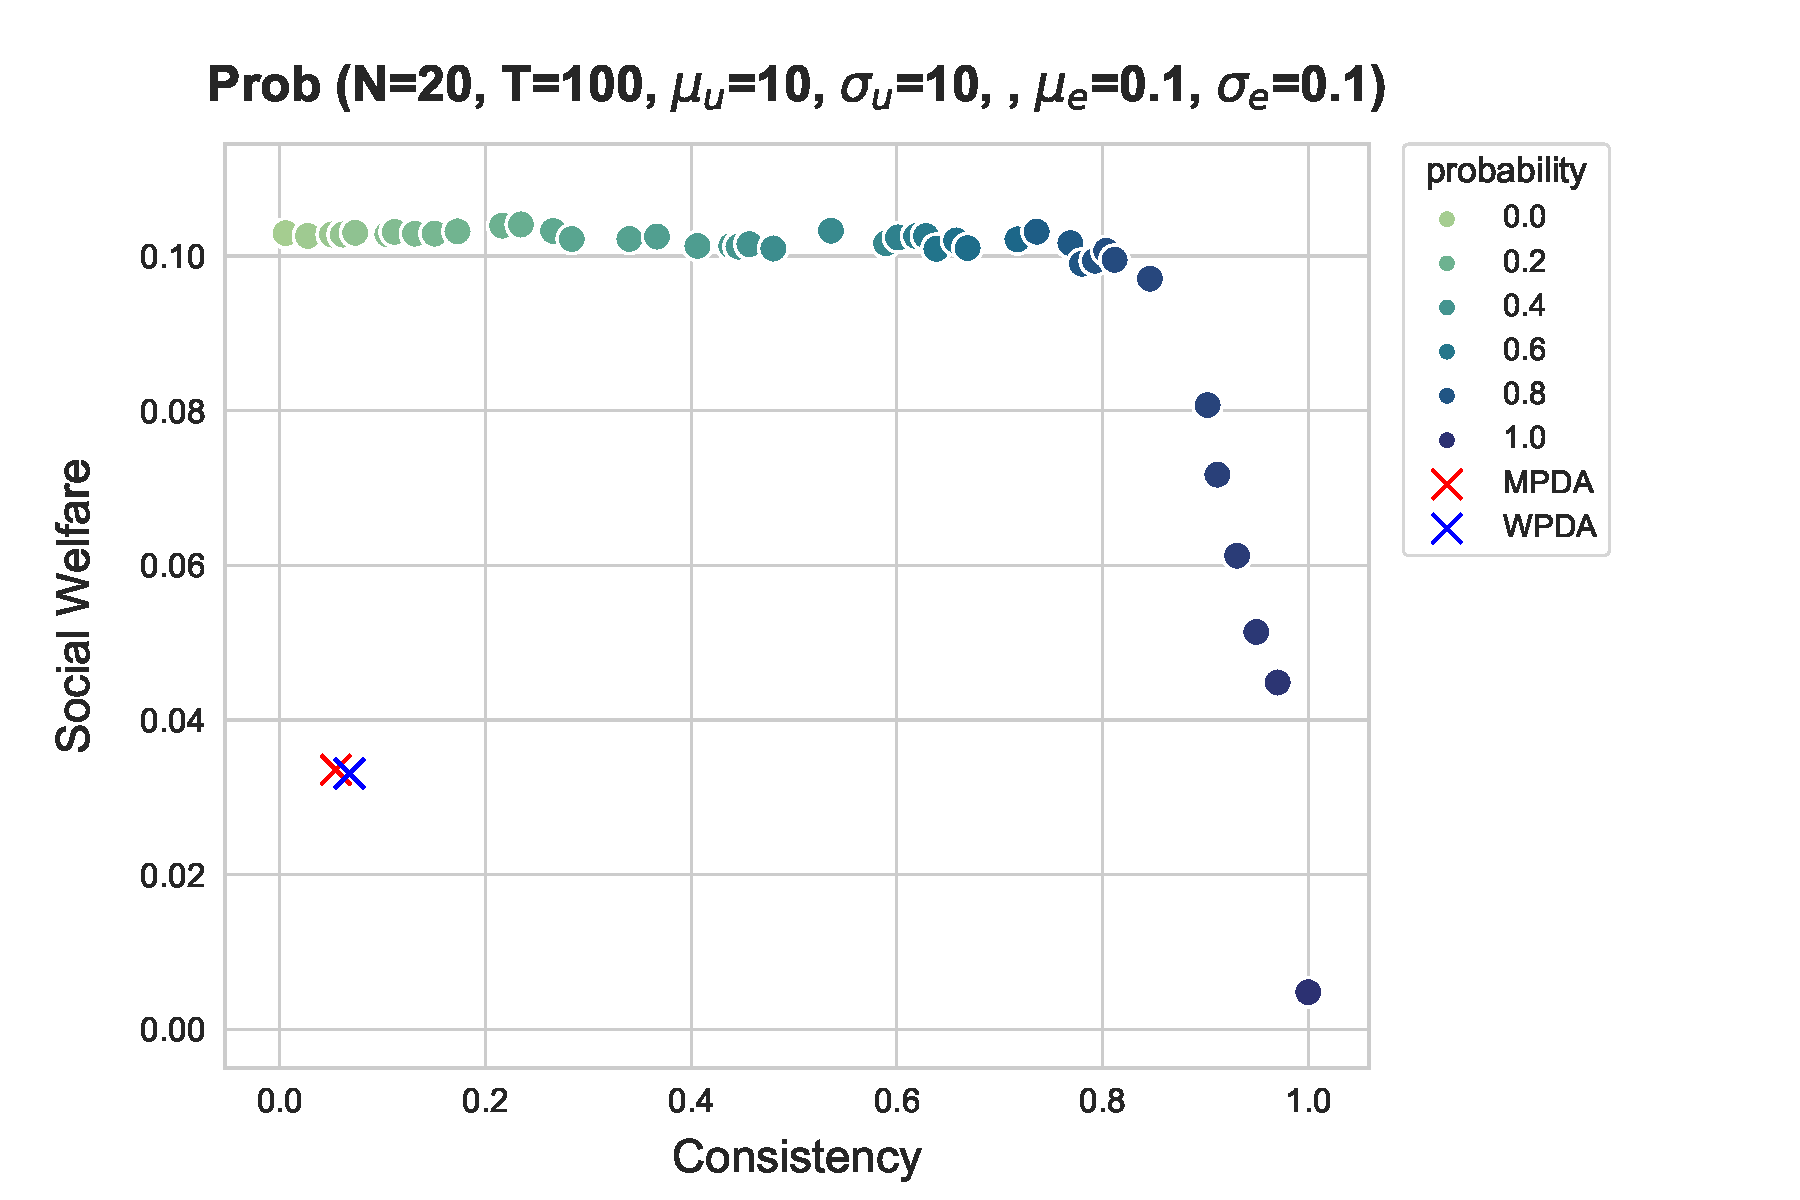
\includegraphics[width=0.32\linewidth]{figures/algs/Prob_20_100_10_10.pdf}
    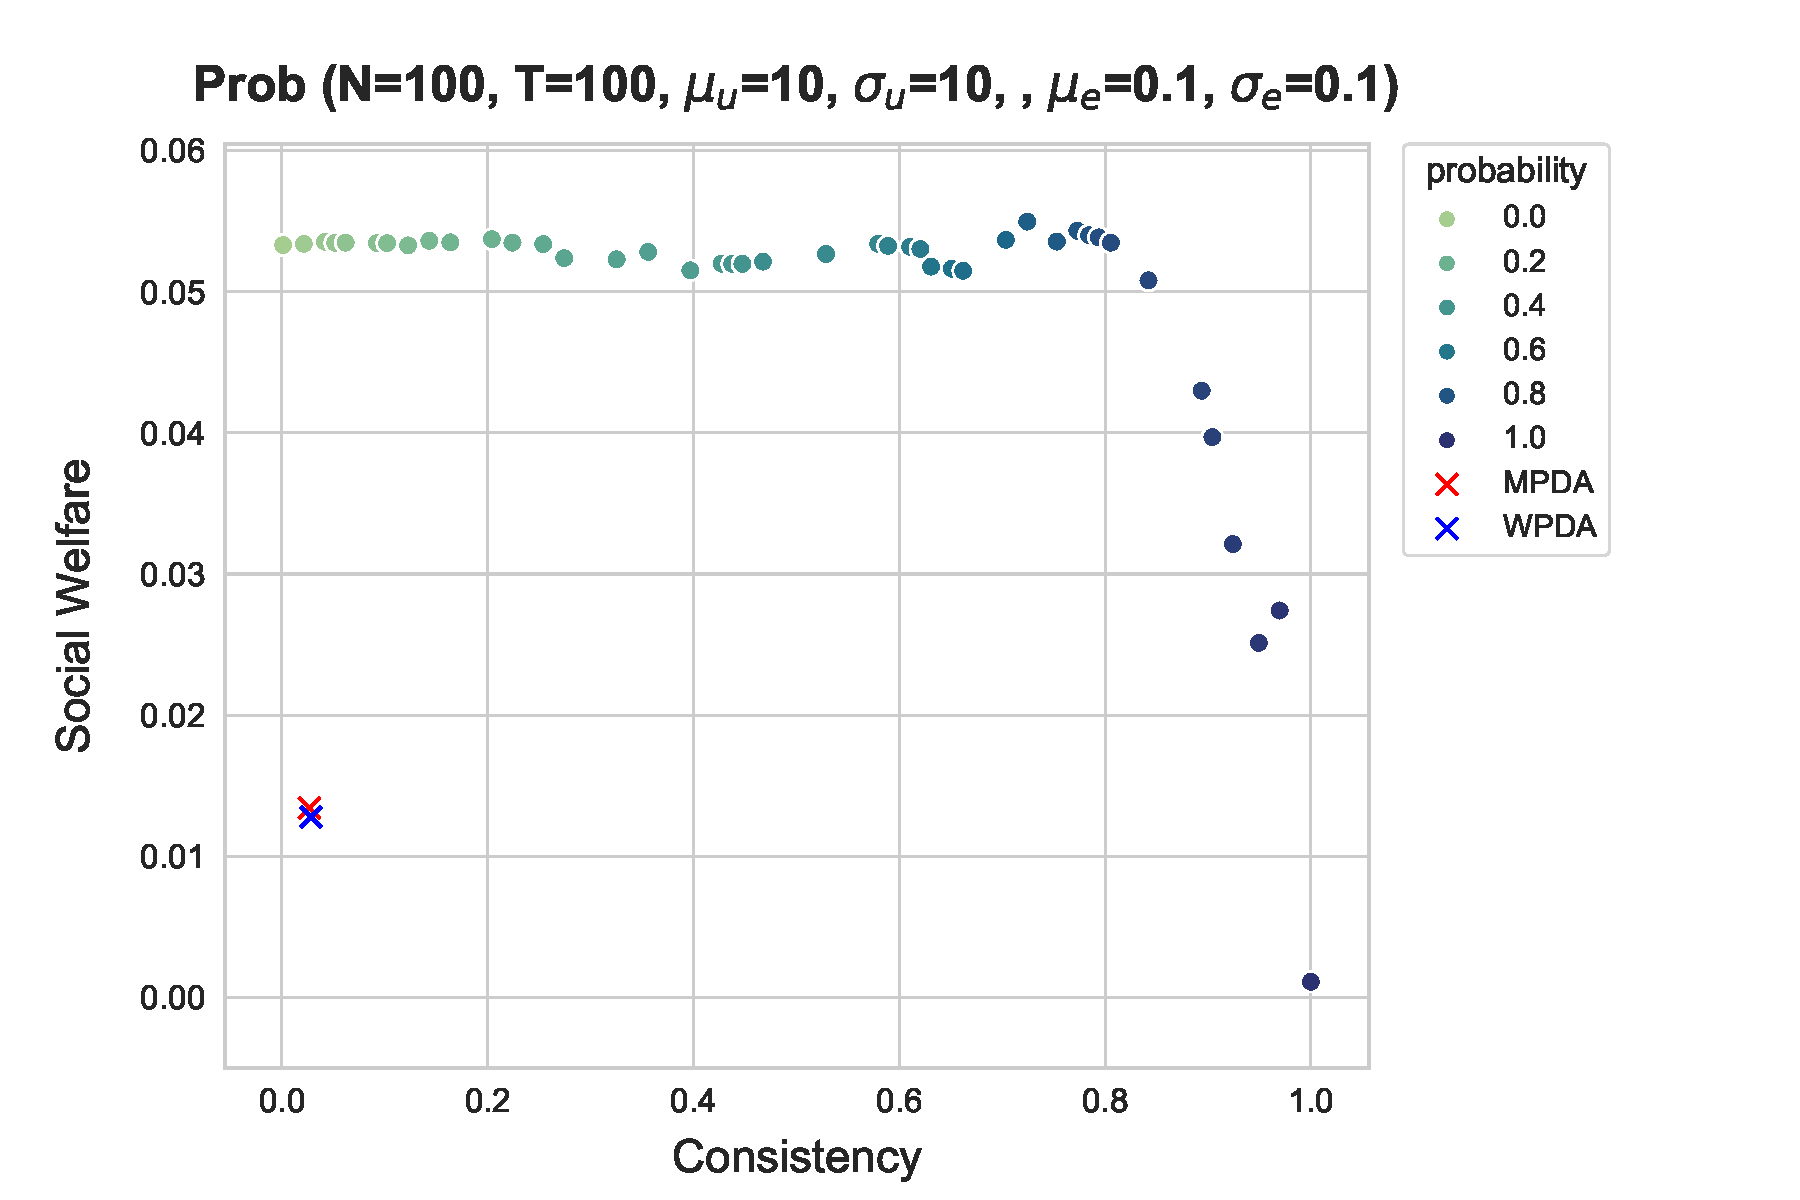
\includegraphics[width=0.32\linewidth]{figures/algs/Prob_100_100_10_10.pdf}
    \caption{Det (top row) and Prob (bottom row) algorithms in the setting where utilities are initialized with $\mathcal{N}(10, 10^2)$ and excitements are initialized with $\mathcal{N}(0.1, 0.1^2)$, with 20 agents and 10 time steps (left column), 20 agents and 100 time steps (middle column), and 100 agents and 100 time steps (right column) respectively.}
    \label{fig:algs}
\end{figure}